\chapter*{Отчёт}
% \section*{Определение $\gamma$-доверительного интервала}
\textbf{Определение} Интервальной оценкой уровня $\gamma \in (0, 1)$ параметра $\theta$ называют пару статистик $\underline{\theta}(\vec{X_n})$ и $\overline{\theta}(\vec{X_n})$ таких, что

$P\{\theta \in (\underline{\theta}(\vec{X}), \overline{\theta}(\vec{X}))\} = \gamma$

\textbf{Определение} $\gamma$-доверительным интервалом (доверительным интервалом уровня $\gamma$) для параметра $\theta$ называется интервал, границы которого отвечают выборочным значениям границ интервальной оценки уровня $\gamma$ для параметра $\theta$:

$(\underline{\theta}(\vec{x}), \overline{\theta}(\vec{x}))$. \newline

%\section*{Формулы для вычисления границ $\gamma$-доверительного интервала}
Формулы для вычисления границ $\gamma$-доверительного интервала для математического ожидания случайной величины:

$\underline{m} = \overline{X} - \frac{S(\vec{X}) u^{(n-1)}_{\frac{1+\gamma}{2}}}{\sqrt{n}}$,

$\overline{m} = \overline{X} + \frac{S(\vec{X}) u^{(n-1)}_{\frac{1+\gamma}{2}}}{\sqrt{n}}$,

где $n$ - объём выборки, 

$\overline{X}$ - выборочное среднее,

$S(\vec{X})$ - точечная оценка диспресии случайной выборки $X$,

$u^{(n-1)}_{\frac{1+\gamma}{2}}$ - квантиль уровня $\frac{1+\gamma}{2}$ распределения Стьюдента с $n-1$ степенями свободы. \newline

Формулы для вычисления границ $\gamma$-доверительного интервала для дисперсии случайной величины:

$\underline{\sigma^2} = \frac{(n-1)S^2(\vec{X})}{h^{(n-1)}_{\frac{1+\gamma}{2}}}$,

$\overline{\sigma^2} = \frac{(n-1)S^2(\vec{X})}{h^{(n-1)}_{\frac{1-\gamma}{2}}}$,

где $n$ - объём выборки, 

$S(\vec{X})$ - точечная оценка диспресии случайной выборки $X$,

$h^{(n-1)}_{\alpha}$ - квантиль уровня $\alpha$ распределения $\chi^2$ с $n-1$ степенями свободы.

\newpage
\section*{Текст программы}
\matlabscript{inc/src/Lab2}{}

\newpage
\section*{Результаты расчетов}

$\stackrel{\wedge}{\mu} = -12.615$,

$S^2 = 0.865$,

$\underline{\mu} = -12.756$,

$\overline{\mu} = -12.474$,

$\underline{\sigma^2} = 0.708$,

$\overline{\sigma^2} = 1.086$.

\section*{Графики}
\begin{figure}[h]
	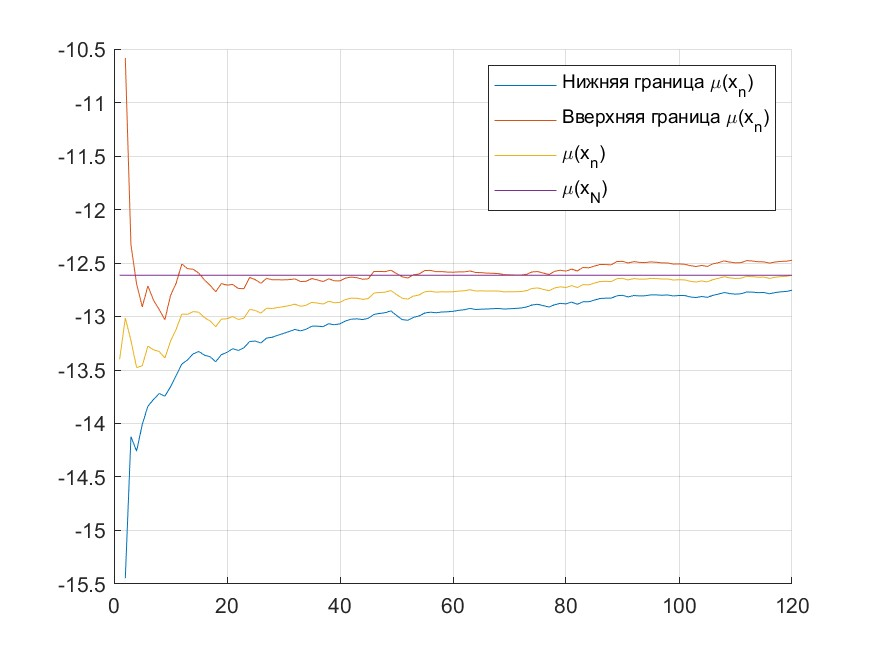
\includegraphics[width=1\linewidth]{inc/img/g1}
	\caption{оценка для математического ожидания}
\end{figure}

\begin{figure}[h]
	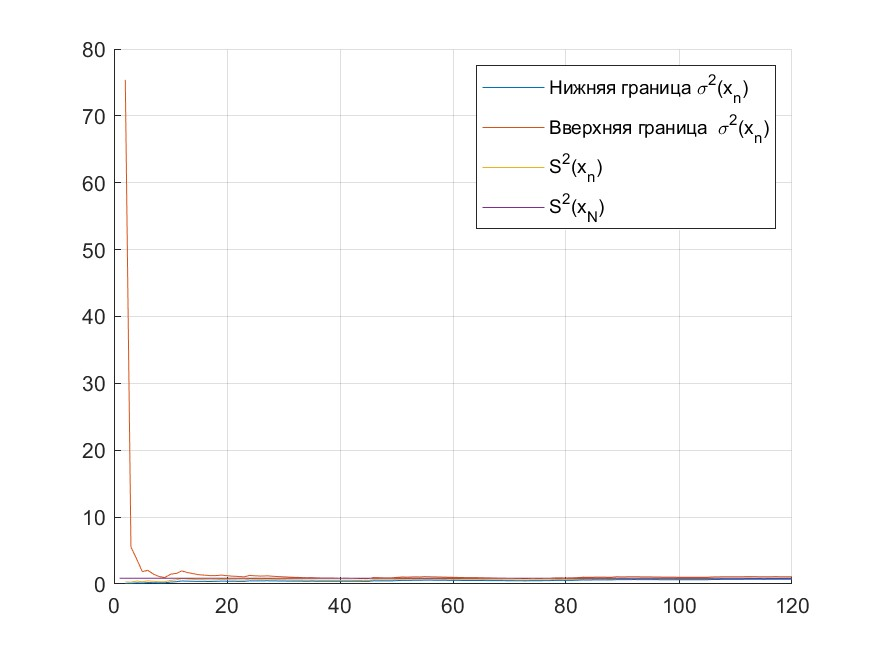
\includegraphics[width=1\linewidth]{inc/img/g2}
	\caption{оценка для дисперсии}
\end{figure}
